
如果您已经学习过复数相关知识,请跳过本页面。

学习复数知识需要一部分向量基础,如果并未学习过向量知识请移步 数学 - 杂项 。

\subsection{复数的引入,定义和分类}

\subsubsection{复数的引入}

注:下面的引入方法来自人教版高中数学 A 版选修 2-2。

我们在实数域中,说 $x^2+1=0$ 这个二次方程无解。这个方程无解,那么我们能不能强行让它有解?如果让它有解的话,确实我们解决了问题,但是这个解的意义是什么?

我们尝试一下,定义一个新数 $\text{i}$,$\text{i}^2+1=0$,那么 $x^2+1=0$ 就有一个解 $x=\text{i}$ 了。

我们希望引入的这个新数与实数域中的数一样,能与实数进行加法和乘法运算,还保留各种运算律。

那么我们很容易想到 $a+b\text{i}$ 这种形式,当然其中 $a,b$ 都是实数。把 $\text{i}$ 看做类似变量的东西,验证其运算性质。我们可以发现,得到的结果全部有着 $a+b\text{i}$ 的类似形式。

那么这样的性质就与实数域类似了,我们把所有有着 $a+b\text{i}$ 形式的数放入一个集合中,就出现了复数集 $\mathbb{C}=\{a+b\text{i} \mid a,b\in \mathbb{R}\}$。

我们可以发现,这个集合中的数和实数集中的数类似,都有在集合中任选两个数进行四则运算,得到的数都是原集合中的数的性质。我们说复数集对于四则运算是\textbf{封闭的}。

\subsubsection{复数的定义和分类}

\begin{QUOTE}{}{}
哇哦我们定义的数的性质这么好!
\end{QUOTE}

我们定义形如 $a+b\text{i}$,其中 $a,b\in \mathbb{R}$ 的数叫做\textbf{复数},其中 $\text{i}$ 被称为\textbf{虚数单位},全体复数的集合叫做\textbf{复数集}。

复数通常用 $z$ 表示,即 $z=a+b\text{i}$。这种形式被称为\textbf{复数的代数形式}。其中 $a$ 称为复数 $z$ 的\textbf{实部},$b$ 称为复数 $z$ 的\textbf{虚部}。如无特殊说明,都有 $a,b\in \mathbb{R}$。

对于一个复数 $z$,当且仅当 $b=0$ 时,它是实数,当 $b\not = 0$ 时,它是虚数,当 $a=0$ 且 $b\not = 0$ 时,它是纯虚数。

纯虚数,虚数,实数,复数的关系如下图所示。

\begin{figure}[htbp]
\centering
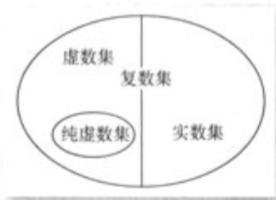
\includegraphics[width=0.7\textwidth]{docs/math/images/complex-1.png} 

\end{figure}



\subsection{复数的性质与运算}

\subsubsection{复数的几何意义}

我们知道了 $a+b\text{i}$ 这样类似的形式的数被称为复数,并且给出了定义和分类,我们还可以挖掘一下更深层的性质。

我们把所有实数都放在了数轴上,并且发现数轴上的点与实数一一对应。我们考虑对复数也这样处理。

首先我们定义\textbf{复数相等}:两个复数 $z_1=a+b\text{i},z_2=c+d\text{i}$ 是相等的,当且仅当 $a=c$ 且 $b=d$。

这么定义是十分自然的,在此不做过多解释。

也就是说,我们可以用唯一的有序实数对 $(a,b)$ 表示一个复数 $z=a+b\text{i}$。这样,联想到平面直角坐标系,我们可以发现\textbf{复数集与平面直角坐标系中的点集一一对应}。好了,我们找到了复数的一种几何意义。

那么这个平面直角坐标系就不再一般,因为平面直角坐标系中的点具有了特殊意义——表示一个复数,所以我们把这样的平面直角坐标系称为\textbf{复平面},$x$ 轴称为\textbf{实轴},$y$ 轴称为\textbf{虚轴}。我们进一步地说:\textbf{复数集与复平面内所有的点所构成的集合是一一对应的}。

我们考虑到学过的平面向量的知识,发现向量的坐标表示也是一个有序实数对 $(a,b)$,显然,复数 $z=a+b\text{i}$ 对应复平面内的点 $Z(a,b)$,那么它还对应平面向量 $\overrightarrow{OZ}=(a,b)$,于是我们又找到了复数的另一种几何意义:\textbf{复数集与复平面内的向量所构成的集合是一一对应的(实数 $0$ 与零向量对应)}。

于是,我们由向量的知识迁移到复数上来,定义\textbf{复数的模}就是复数所对应的向量的模。复数 $z=a+b\text{i}$ 的模 $|z|=\sqrt{a^2+b^2}$。

于是为了方便,我们常把复数 $z=a+b\text{i}$ 称为点 $Z$ 或向量 $\overrightarrow {OZ}$,并规定相等的向量表示同一个复数。

并且由向量的知识我们发现,虚数不可以比较大小(但是实数是可以的)。

\subsubsection{复数的运算}

\paragraph{复数的加法与减法}

我们规定,复数的加法规则如下:

设 $z_1=a+b\text{i},z_2=c+d\text{i}$,那么

$$
z_1+z_2=(a+c)+(b+d)\text{i}
$$

很明显,两个复数的和仍为复数。

考虑到向量的加法运算,我们发现复数的加法运算符合向量的加法运算法则,这同样证明了复数的几何意义的正确性。

同样可以验证,\textbf{复数的加法满足交换律和结合律}。即:

$$
z_1+z_2=z_2+z_1\\
(z_1+z_2)+z_3=z_1+(z_2+z_3)
$$

减法作为加法的逆运算,我们可以通过加法法则与复数相等的定义来推导出减法法则:

$$
z_1-z_2=(a-c)+(b-d)\text{i}
$$

这同样符合向量的减法运算。

\paragraph{复数的乘法与除法}

我们规定,复数的加法规则如下:

设 $z_1=a+b\text{i},z_2=c+d\text{i}$,那么

$$
\begin{aligned}
z_1z_2&=(a+b\text{i})(c+d\text{i})\\
&=ac+bc\text{i}+ad\text{i}+bd\text{i}^2\\
&=(ac-bd)+(bc+ad)\text{i}
\end{aligned}
$$

可以看出,两个复数相乘类似于两个多项式相乘,只需要把 $\text{i}^2$ 换成 $-1$,并将实部与虚部分别合并即可。

复数确实与多项式有关,因为复数域是实系数多项式环模掉 $x^2+1$ 生成的理想。(这句话不明白其实也没有关系)

复数的乘法与向量的向量积形式类似,是由于复数集是数环。

于是容易知道,\textbf{复数乘法满足交换律,结合律和对加法的分配律},即:

$$
z_1z_2=z_2z_1\\
(z_1z_2)z_3=z_1(z_2z_3)\\
z_1(z_2+z_3)=z_1z_2+z_1z_3
$$

由于满足运算律,我们可以发现实数域中的\textbf{乘法公式在复数域中同样适用}。

除法运算是乘法运算的逆运算,我们可以推导一下:

$$
\begin{aligned}
\frac{a+b\text{i}}{c+d\text{i}}&=\frac{(a+b\text{i})(c-d\text{i})}{(c+d\text{i})(c-d\text{i})}\\
&=\frac{ac+bd}{c^2+d^2}+\frac{bc-ad}{c^2+d^2}\text{i} &(c+d\text{i}\not =0)
\end{aligned}
$$

为了分母实数化,我们乘了一个 $c-d\text{i}$,这个式子很有意义。

我们定义,当两个虚数实部相等,虚部互为相反数时,这两个复数互为\textbf{共轭复数}。通常记 $z=a+b\text{i}$ 的共轭复数为 $\bar z=a-b\text{i}$。我们可以发现,两个复数互为共轭复数,那么它们\textbf{关于实轴对称}。

由于向量没有除法,这里不讨论与向量的关系。
